\documentclass[11pt, a4paper]{article}
\usepackage[a4paper, margin=2.0cm]{geometry}
\usepackage{amsmath, amssymb}
\usepackage{graphicx}
\usepackage{booktabs}
\usepackage{tabularx}
\usepackage{array}
\usepackage{float}
\usepackage{caption}
\usepackage{subcaption}
\usepackage{listings}
\usepackage[hidelinks]{hyperref}

\graphicspath{{../results/mid/figures/}{../results/mid/figures/qualitative/}}
\captionsetup{font=small, labelfont=bf}
\lstset{basicstyle=\ttfamily\small, frame=single, columns=fullflexible, keepspaces=true,
        showstringspaces=false, breaklines=true, xleftmargin=4pt, xrightmargin=4pt}
\setlength{\parskip}{4pt}
\renewcommand{\arraystretch}{1.1}

\title{\textbf{Calibrated Confidence for Kilometre-Scale Feed-Forward SLAM}\\[4pt]
\large Mid-Submission Report, Mobile Robotics (Monsoon 2026)}
\author{Kavish Vora \quad Pranav Srivastava \quad Mehrish Khan\\ IIIT Hyderabad}
\date{}

\begin{document}
\maketitle

\noindent This report covers the work done so far: the tasks completed, the objectives achieved,
the experimental results and metrics obtained so far, and the plan for the rest of the project. We test whether
VGGT's per-pixel confidence \cite{vggt} can tell VGGT-Long \cite{vggtlong} how much to trust each joint between
windows (seams) and each loop closure, and whether weighting the pose graph with calibrated confidence improves the
trajectory.

\section{Tasks completed}

Table~\ref{tab:tasks} lists every task planned for the mid submission and what was done. All runs used KITTI
\cite{kitti} sequences 05 and 07 for fitting (everything learned is learned there) and 00 and 02 as held-out test
sequences.

\begin{table}[!t]
\centering
\caption{Mid-submission tasks and what was done.}
\label{tab:tasks}
\small
\begin{tabularx}{\textwidth}{>{\raggedright\arraybackslash}p{4.1cm} X}
\toprule
Task & What we did \\
\midrule
Data and conventions &
KITTI images, ground-truth poses, calibration and the 13{,}064 LiDAR scans of 00, 02, 05, 07. Ground truth converted
from camera 0 to the colour camera 2 that VGGT sees; LiDAR projected onto VGGT's 518$\times$154 input grid and checked
visually. \\
VGGT set-up and memory test &
VGGT-1B on one RTX A4000 (16\,GB, bfloat16). Memory and speed measured for windows of 8 to 64 frames. Four automatic
convention checks (smoke test) passed before the long runs. \\
Run VGGT on all sequences &
814 windows of 32 frames with 16 frames overlap, plus 43 loop windows. \\
Reproduce VGGT-Long &
(i) Our own back end (alignment, loops, pose graph) checked against VGGT-Long's code piece by piece. (ii) The original
\texttt{vggt\_long.py} run on all four sequences at window/overlap 30/15 and 60/30 (the paper's settings), 32/16 (ours)
and 75/30 (released default): 16 runs; plus checks on 02 (another code version, more optimiser iterations, 90/45). \\
True error of every seam and loop &
For every window, the Sim(3) that places its predicted cameras on the ground truth; the true 7-number error of each edge
follows from these. 834 of 853 edges usable (windows where the car is nearly stopped are skipped). \\
Pixel confidence audit &
LiDAR depth compared with the depth head and the point head after one scale per window: 478 million
(confidence, error) pairs. \\
Calibration on 05/07 &
Pixel level: raw $1/C$ rule; the two-constant power law from the calibration audit of feed-forward 3D reconstruction
models by N.~Deng et al.~\cite{dengaudit}; isotonic curve. Edge level: isotonic map from an edge feature to the expected
squared error of rotation, translation and scale. \\
Weighting schemes (a) to (g) on 00/02 &
Seven schemes plus a control (a$'$), each without loops, with loops, and with a robust kernel on loop edges: Huber, or
Dynamic Covariance Scaling (DCS) by Agarwal et al.~\cite{dcs}; thresholds tuned on 05/07. \\
Ground truth at loop revisits &
LiDAR scans of both visits of every loop placed with the ground-truth poses, to check whether the ground truth itself
is consistent where the car comes back. \\
Tables, figures, qualitative results &
All tables and 45 figures produced by one command from the saved outputs. \\
\bottomrule
\end{tabularx}
\end{table}

\noindent The schemes differ only in how much each edge of the pose graph is trusted:
(a) VGGT-Long's equal weights, with VGGT-Long's own way of measuring an edge's mismatch (the reproduction anchor);
(a$'$) equal weights with the mismatch measure used by all other schemes, the fair control for (b) to (g);
(b) one fitted variance each for rotation, translation (relative to the window's depth) and scale, with a separate fitted
factor for loops, but no per-edge information; (c) (b) scaled by the square of the edge's mean confidence;
(d) the alignment residual only (no confidence); (e) our calibrated confidence;
(f) an oracle using each edge's true error (a reference, not a method); (g) the per-pixel power law from ``A calibration
audit of confidence in feed-forward 3D reconstruction models'' by N.~Deng et al.~\cite{dengaudit}.
An edge's weight is the inverse of its predicted variance, block by block:
\begin{lstlisting}
info[:, :3]  = 1 / var_rot              # rotation (3 numbers)
info[:, 3:6] = 1 / (var_trans * L**2)   # translation (3 numbers); L: typical depth
info[:, 6]   = 1 / var_scale            # scale (1 number)
\end{lstlisting}

\section{Objectives achieved}

\begin{itemize}
  \item \textbf{Data, model and conventions verified.} All four smoke-test checks passed (depth head and point head agree;
        the first camera of each window is the identity; cameras match ground truth after one Sim(3); poses are
        camera-to-world).
  \item \textbf{VGGT-Long reproduced.} The original code matches the paper within 0.5\% at the paper's 30/15 setting on all
        four sequences, and our re-implementation matches the original code within 0.7\% at 32/16. Both loop finders
        return identical loop pairs on all four sequences.
  \item \textbf{Confidence audit done.} True errors for all usable seams and loops, and a confidence audit on 478 million
        LiDAR pixels for both heads.
  \item \textbf{End-to-end baseline ready.} Calibration fitted on 05/07; all seven schemes, with and without loops and robust
        kernels, evaluated on 00/02; first tables and figures.
\end{itemize}

\section{Experimental results and metrics}

\paragraph{Metrics.} \textbf{ATE}: root-mean-square distance between estimated and true camera positions after the best
rotation, shift and scale (Umeyama alignment \cite{umeyama}), in metres. \textbf{t\_rel}: KITTI's average translation
drift (\%) over 100 to 800\,m segments. For uncertainty: the \textbf{ratio} of mean squared error to mean predicted
variance (1 is perfect), a binned \textbf{calibration error} (0 is perfect), \textbf{NEES} (7 is perfect for 7 numbers)
and \textbf{coverage} of the predicted 95\% region (0.95 is perfect). Our ATE equals the evo tool \cite{evo} on all 72
trajectories (largest difference $10^{-9}$\,m).

\subsection{Data and running cost}

\begin{table}[H]
\centering
\caption{Sequences used and VGGT's cost. LiDAR pixels count each LiDAR point once per window containing its frame.}
\label{tab:data}
\small
\begin{tabular}{lcrrrrrr}
\toprule
Seq. & Role & Frames & Windows & Loops & Usable edges & LiDAR pixels & Frames / s \\
\midrule
05 & fit  & 2761 & 172 & 12 & 176 / 183 & 101.3\,M & 17.4 \\
07 & fit  & 1101 &  68 &  3 &  62 / 70  &  39.1\,M & 17.4 \\
00 & test & 4541 & 283 & 20 & 298 / 302 & 163.5\,M & 17.3 \\
02 & test & 4661 & 291 &  8 & 298 / 298 & 174.4\,M & 17.2 \\
\bottomrule
\end{tabular}
\end{table}

\noindent One VGGT pass on the A4000 needs 7.7, 8.4, 9.0, 9.6, 10.9 and 12.2\,GB for windows of 8, 16, 24, 32, 48 and 64
frames; a 32-frame window takes 1.8\,s. The original VGGT-Long code took 5 to 6 minutes for 07 and 18 to 26 minutes for 00
and 02 per setting.

\subsection{Reproduction of VGGT-Long}

\begin{table}[H]
\centering
\caption{ATE (m). Paper: Table 1 of \cite{vggtlong}. Original code: \texttt{vggt\_long.py} run by us. Ours (a): our
re-implementation with VGGT-Long's equal weights.}
\label{tab:repro}
\small
\begin{tabular}{llrrrr}
\toprule
Source & Window / overlap & 05 & 07 & 00 & 02 \\
\midrule
Paper          & 30 / 15 & 10.20 & 4.00 & 9.06 & 99.95 \\
Original code  & 30 / 15 & 10.24 & 3.98 & 9.07 & 99.65 \\
Original code  & 32 / 16 & 10.04 & 4.09 & 9.13 & 104.61 \\
\textbf{Ours (a)} & 32 / 16 & \textbf{10.02} & \textbf{4.06} & \textbf{9.18} & \textbf{105.07} \\
\midrule
Paper          & 60 / 30 & 9.15 & 2.68 & 8.06 & 34.16 \\
Original code  & 60 / 30 & 9.85 & 2.66 & 8.63 & 52.78 \\
Original code  & 75 / 30 & 10.15 & 2.84 & 10.83 & 55.90 \\
\midrule
Paper          & 90 / 45 & 9.88 & 3.47 & 11.97 & 49.85 \\
Original code  & 90 / 45 & -- & -- & -- & 50.56 \\
\bottomrule
\end{tabular}
\end{table}

\noindent The original code reproduces the paper within 0.5\% at 30/15, and our version matches the original code within
0.7\% at 32/16 (Figure~\ref{fig:upstream}), so our baseline is VGGT-Long itself. The large error on 02 with small windows is
also in the paper. At 60/30 our runs are within 8\% of the paper on 05, 07 and 00. On 02 at 60/30 we get 52.78\,m where the
paper reports 34.16\,m, although the same code matches the paper on 02 at 30/15 and 90/45 (99.65 against 99.95\,m, 50.56
against 49.85\,m). An October 2025 version of the code, 200 instead of 30 iterations of its loop optimiser, and its older
loop threshold all give exactly 52.78\,m, so we could not reproduce this one number.

\begin{figure}[H]
\centering
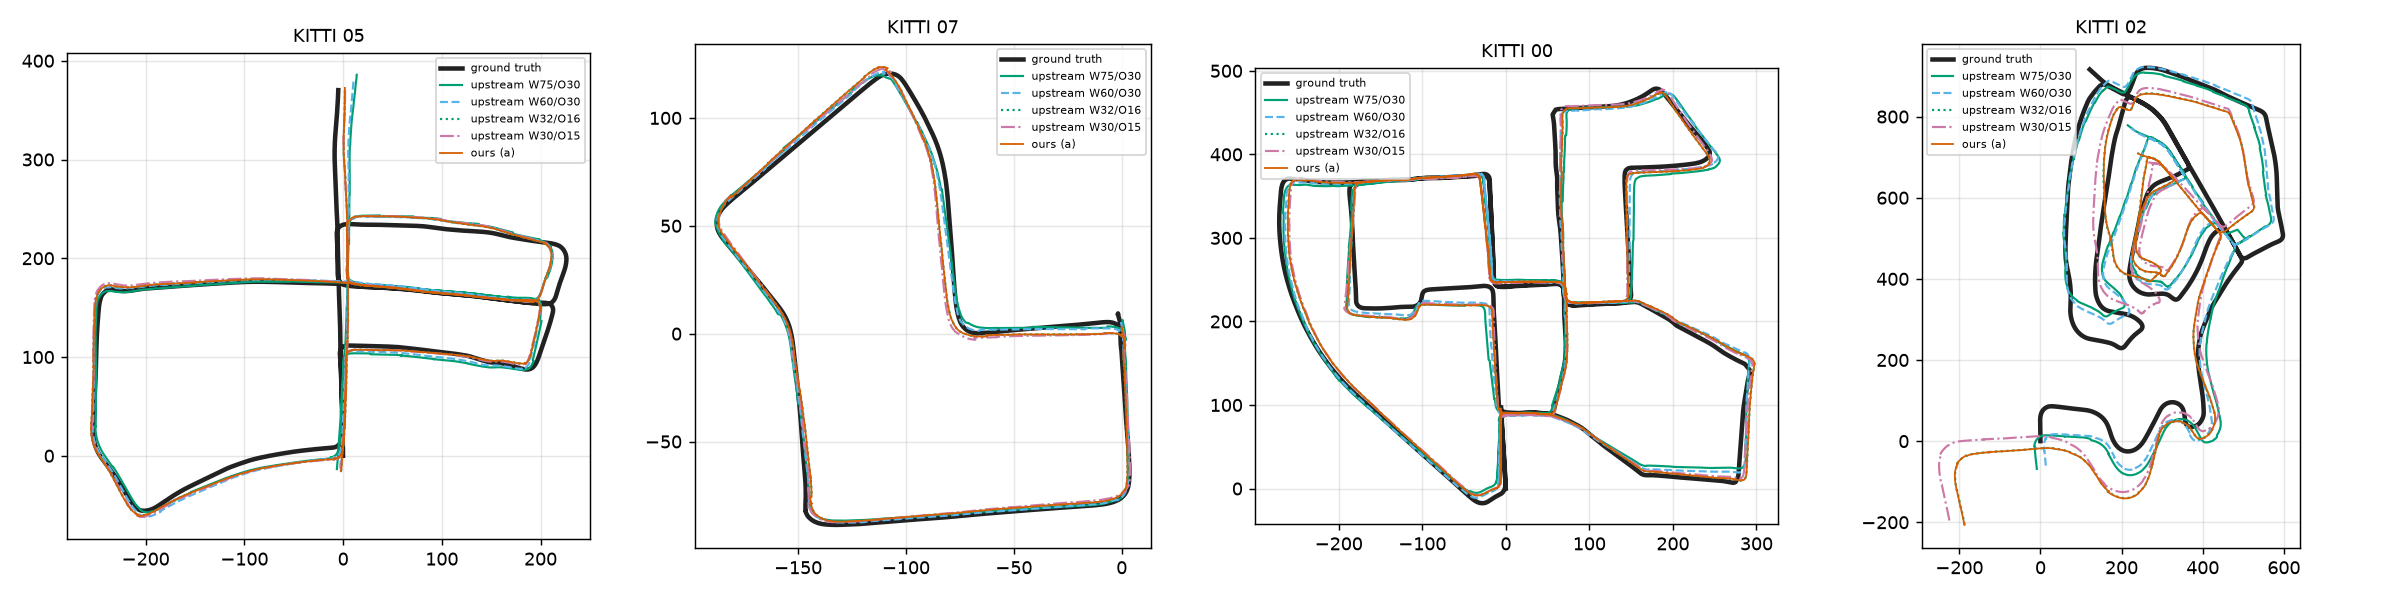
\includegraphics[width=\textwidth]{upstream_vs_ours.png}
\caption{Top view of the trajectories (m) after Sim(3) alignment: ground truth (black), the original VGGT-Long code at four
settings and our version (a) at 32/16, which lies on top of the original code at the same setting.}
\label{fig:upstream}
\end{figure}

\subsection{Pixel confidence against LiDAR}

\begin{table}[H]
\centering
\caption{Held-out sequences (00, 02). Slope of log(error) against log(confidence): $-1$ would match the simple rule
error $\propto 1/C$. Calibration error: 0 is perfect. Fitted on 140 million pixels of 05/07.}
\label{tab:pixel}
\small
\begin{tabular}{lrrrrrr}
\toprule
Head & Pixels & Slope & Spearman & Raw $\kappa/C$ & Power law & Isotonic \\
\midrule
Depth head & 337.9\,M & $-0.70$ & $-0.34$ & 0.40 & 0.25 & \textbf{0.18} \\
Point head & 337.9\,M & $-0.63$ & $-0.40$ & 0.60 & 0.53 & \textbf{0.32} \\
\bottomrule
\end{tabular}
\end{table}

\begin{figure}[H]
\centering
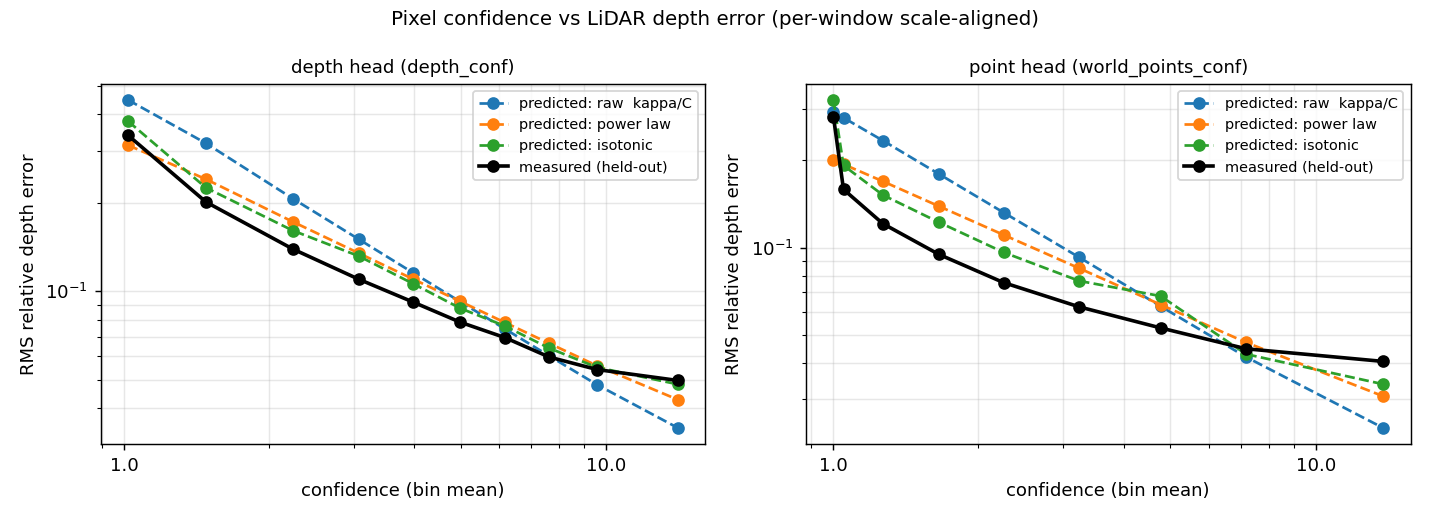
\includegraphics[width=0.88\textwidth]{pixel_calibration.png}
\caption{Root-mean-square depth error per confidence bin on 00 and 02 (black) and what each predictor expects. Higher
confidence does mean lower error, but less steeply than $1/C$; the isotonic curve fitted on 05/07 follows the data best.}
\label{fig:pixel}
\end{figure}

\noindent Confidence ranks pixel errors correctly but understates how slowly the error falls (slope $-0.7$, not $-1$).
A monotone calibration learned on other sequences removes most of the mismatch (0.40 to 0.18 for the depth head). The
largest errors sit on object borders, which also get low confidence (Figure~\ref{fig:depth}).

\begin{figure}[H]
\centering
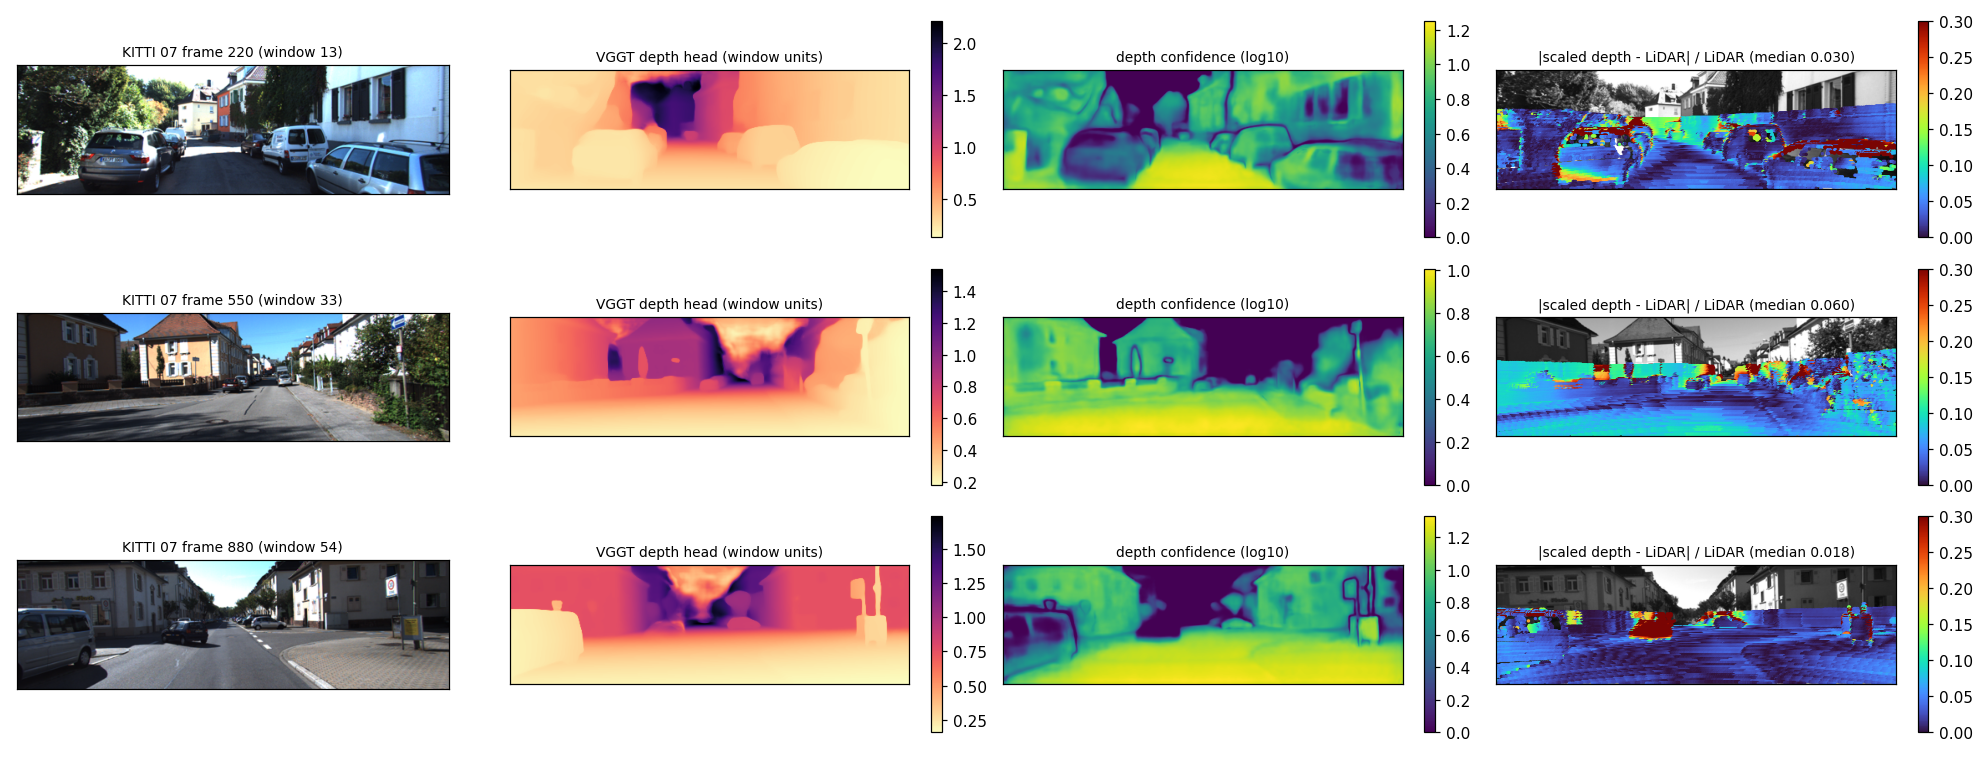
\includegraphics[width=\textwidth]{depth_lidar_07.png}
\caption{KITTI 07, three frames. From left: image, VGGT depth, depth confidence (log), and relative depth error at LiDAR
pixels after scale alignment (median 2 to 6\%; high on object borders).}
\label{fig:depth}
\end{figure}

\subsection{Seams and loops}

\begin{table}[H]
\centering
\caption{Predicted uncertainty against true error on the held-out edges, before rescaling. Ratio: mean squared error over
mean predicted variance (1 is perfect, above 1 is over-confident). NEES: 7 is perfect. Coverage: share of edges inside the
predicted 95\% region (0.95 is perfect). The loop rows use loop labels that include ground-truth height errors on 00
and 02 (see Loops below).}
\label{tab:edges}
\small
\begin{tabular}{llrrrrr}
\toprule
& & \multicolumn{3}{c}{Ratio} & & \\
\cmidrule(lr){3-5}
Edges & Scheme & rotation & translation & scale & NEES & Coverage \\
\midrule
569 seams & (b) uniform        & 1.36 & 1.32 & 1.29 &  9.3 & 0.80 \\
          & (c) raw confidence & 0.90 & 0.87 & 0.85 &  7.7 & 0.86 \\
          & (d) geometry only  & 1.44 & 1.40 & 1.33 & 11.0 & 0.77 \\
          & (e) calibrated     & 1.29 & 1.26 & 1.29 & 11.5 & 0.76 \\
          & (g) power law      & 1.57 & 1.07 & 1.04 &  9.9 & 0.78 \\
\midrule
27 loops  & (b) uniform        & 2.00 & 22.36 &  9.78 &  82.9 & 0.11 \\
          & (e) calibrated     & 1.58 & 23.27 & 10.70 & 119.8 & 0.15 \\
          & (g) power law      & 0.26 &  4.63 &  0.65 &  25.3 & 0.63 \\
\bottomrule
\end{tabular}
\end{table}

\noindent \textbf{Seams.} All schemes predict the right size of seam error within a factor of about 1.5. Ranking is weaker
(Table~\ref{tab:rank}): a seam's mean confidence ranks its rotation error (Spearman $-0.44$) but hardly its translation
error ($-0.12$); the alignment residual ranks translation best ($0.55$). The worst seams look at vegetation or are taken
during turns, where confidence is low almost everywhere (Figure~\ref{fig:seams}).

\begin{table}[H]
\centering
\caption{Spearman rank correlation between a seam feature and the seam's true error (569 held-out seams). For confidence,
negative means ``more confident, smaller error'', the desired direction.}
\label{tab:rank}
\small
\begin{tabular}{lrrr}
\toprule
Feature & rotation & translation & scale \\
\midrule
Mean confidence    & $-0.44$ & $-0.12$ & $-0.10$ \\
Median confidence  & $-0.26$ & $-0.13$ & $-0.03$ \\
Alignment residual & $0.24$  & $\mathbf{0.55}$ & $0.30$ \\
Inlier fraction    & $-0.17$ & $-0.25$ & $-0.20$ \\
\bottomrule
\end{tabular}
\end{table}

\begin{figure}[H]
\centering
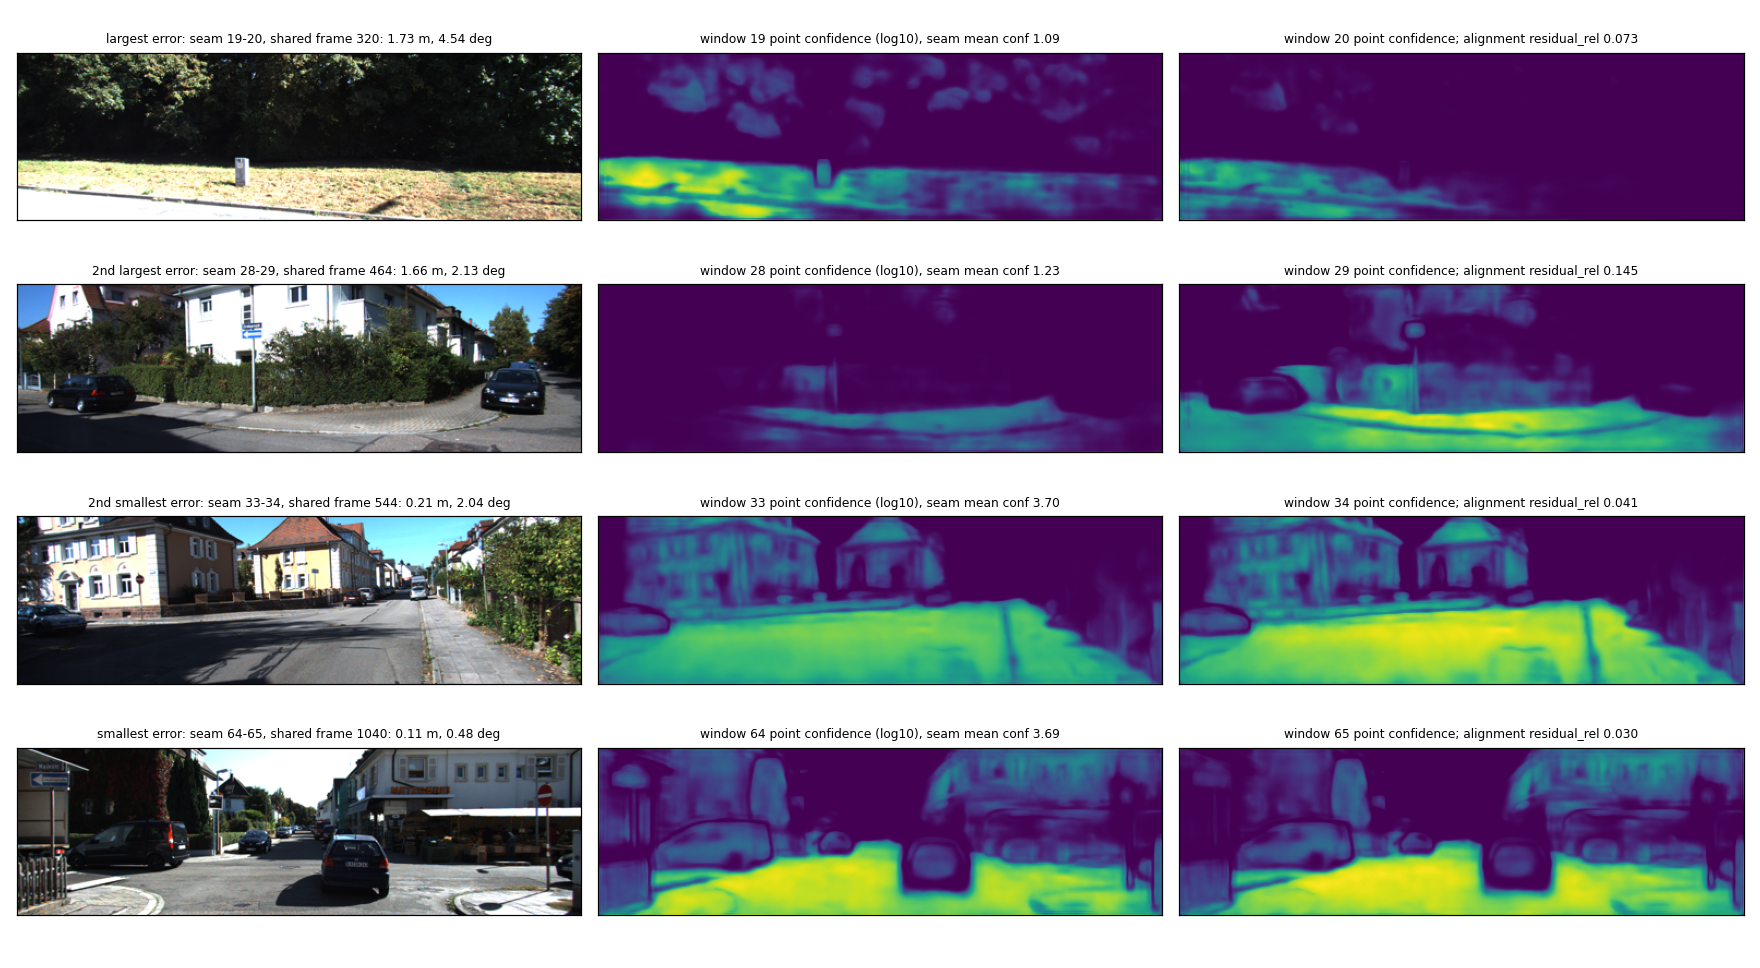
\includegraphics[width=\textwidth]{seams_07.png}
\caption{KITTI 07, the two worst and two best seams by true error: shared frame (left) and point confidence of the two
windows (log scale). Bad seams see hedges or turn corners with low confidence; good seams see buildings and road.}
\label{fig:seams}
\end{figure}

\noindent \textbf{Loops.} We checked all 43 loops, and every one is a real revisit of the same place. On held-out loops the
measured squared errors are about 20 times larger than predicted (about 4.7 times in error size). When we looked at where
the loop errors come from, we found that the ground truth itself is not consistent at the revisits of 02 and, less so,
00: the two visits of the same road are placed 1 to 4\,m apart \emph{in height} (Table~\ref{tab:loops}). To check this
independently, we placed the LiDAR scans of both visits with the ground-truth poses and compared the road surface at the
same spot. A road cannot be at two heights at once, yet the two road surfaces end up 0.8 to 4.1\,m apart on 02, matching
the ground-truth gap almost exactly, while on 05 and 07 they agree to within 0.2\,m (0.5\,m for two loops of 05). So on 02 the ground-truth heights at
the revisits are off by up to 4\,m, and most of what we measured as loop error there is error in the ground truth, not
in VGGT (Figure~\ref{fig:loops}). Seam errors are not affected, because each seam only uses the ground truth within one
short window.

\begin{table}[H]
\centering
\caption{Loops per sequence (medians, maxima in brackets). GT gap: distance between the two visits in the ground truth,
and its vertical part. Road gap: height difference between the two visits' LiDAR road surfaces at the same spot after
placing both with the ground truth (0 if the ground truth is consistent). Edge error: measured translation error of the
loop edge.}
\label{tab:loops}
\small
\begin{tabular}{lrrrrr}
\toprule
Seq. & Loops (usable) & GT gap (m) & GT vertical gap (m) & LiDAR road gap (m) & Edge error (m) \\
\midrule
05 & 12 (10) & 0.31 (0.81) & 0.05 (0.50) & 0.05 (0.52) & 0.37 (1.13) \\
07 &  3 (1)  & 0.41 (0.52) & 0.12 (0.16) & 0.18 (0.21) & 0.97 (0.97) \\
00 & 20 (19) & 0.67 (2.06) & 0.47 (1.07) & 0.49 (1.30) & 1.16 (2.15) \\
02 &  8 (8)  & 2.64 (4.09) & 1.94 (4.01) & 2.02 (4.06) & 3.05 (6.18) \\
\bottomrule
\end{tabular}
\end{table}

\begin{figure}[H]
\centering
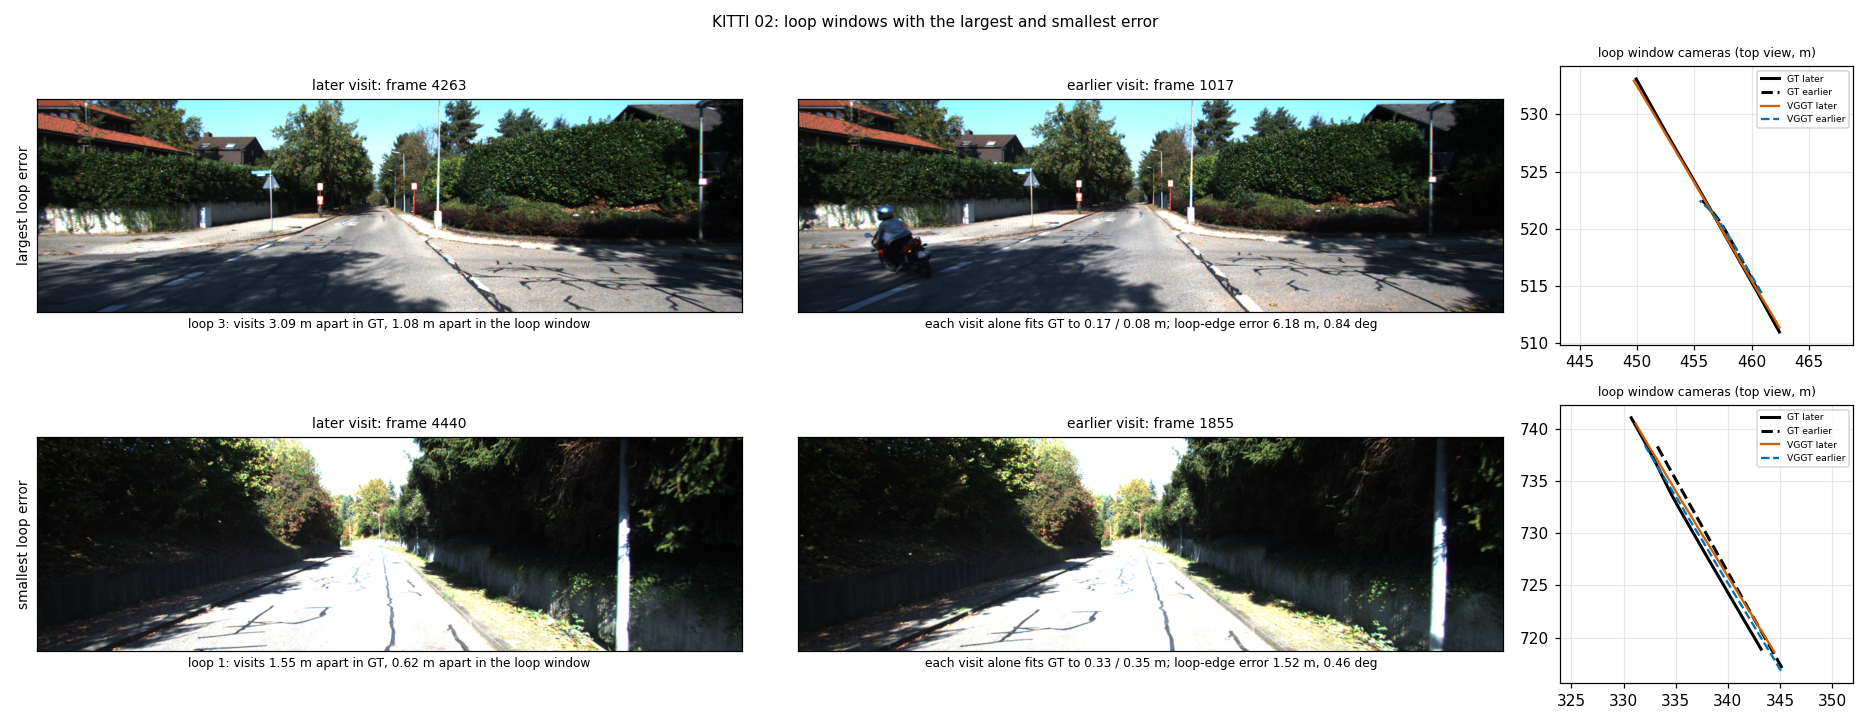
\includegraphics[width=\textwidth]{loops_02.png}
\caption{KITTI 02, the loops with the largest and smallest measured error. Top: the ground truth places the two visits
3.09\,m apart, almost all of it in height, while VGGT's loop window puts them 1.08\,m apart; the LiDAR road surfaces of
the two visits, placed with the ground truth, are 3.09\,m apart in height, so the ground truth is inconsistent here.}
\label{fig:loops}
\end{figure}

\subsection{Trajectories}

\begin{table}[H]
\centering
\caption{ATE (m) / t\_rel (\%) with loops, window 32/16. Robust kernels change these numbers only where noted below.
$^*$The oracle uses the true edge errors and is not a method.}
\label{tab:traj}
\small
\begin{tabular}{lcccc}
\toprule
Weighting & 05 (fit) & 07 (fit) & 00 (test) & 02 (test) \\
\midrule
No loops (any scheme) & 48.70 / 13.78 & 22.36 / 13.30 & 140.49 / 34.47 & 181.52 / 40.90 \\
\midrule
(a) VGGT-Long         & 10.02 / 5.11 & 4.06 / 3.94 & 9.18 / 4.82 & \textbf{105.07 / 26.95} \\
(a$'$) equal, control  & 9.80 / 5.05 & 4.07 / 3.93 & 9.14 / 4.74 & 106.90 / 27.45 \\
\midrule
(b) uniform         & 11.52 / 5.83 & \textbf{3.61 / 3.53} & 10.15 / 4.88 & 113.36 / 29.81 \\
(c) raw confidence    & 10.05 / 5.12 & 4.55 / 3.84 & 10.28 / 5.03 & 119.60 / 31.44 \\
(d) geometry only     & 11.10 / 5.49 & 4.49 / 3.88 & 9.34 / 4.75 & 113.27 / 29.86 \\
(e) calibrated (ours) & 9.57 / 4.78 & 4.37 / 3.83 & \textbf{9.09 / 4.68} & 117.07 / 30.59 \\
(f) oracle$^*$        & \textbf{8.94 / 4.30} & 4.59 / 4.17 & 11.92 / 5.31 & 116.08 / 29.56 \\
(g) power law         & 10.39 / 5.24 & 4.37 / 3.79 & 9.89 / 4.89 & 119.70 / 31.47 \\
\bottomrule
\end{tabular}
\end{table}

\noindent Kernel effects: Huber never down-weighted a loop and changes ATE by at most 0.04\,m. DCS switched off all 8 (true)
loops on 02 for schemes (b), (c), (d) and (g), raising their ATE to about 175\,m, close to the no-loop result. The main
observations:
\begin{itemize}
  \item \textbf{Loops matter most:} they cut the error 5 to 15 times (00: 140\,m to 9\,m).
  \item \textbf{Weighting matters less:} compared with the fair control (a$'$), our calibrated scheme (e) is better on 05
        (9.57\,m against 9.80\,m) and 00 (9.09\,m against 9.14\,m) but worse on 07 and 02. Schemes differ by 10 to 25\% on a
        given sequence. The way an edge's mismatch is measured alone changes ATE by up to 2\% ((a) against (a$'$)).
  \item \textbf{On 02 every weighted scheme is worse than equal weights.} We have not yet isolated why; the loop labels on 02
        are affected by ground-truth height errors (previous section), which also affects every scheme fitted from labels.
  \item \textbf{The oracle is not the best either.} This shows only that weighting each edge by its own measured error is
        not an upper bound here, not that per-edge weighting cannot help; on 02 its loop errors also include the
        ground-truth height errors.
\end{itemize}

\begin{figure}[H]
\centering
\begin{subfigure}{0.49\textwidth}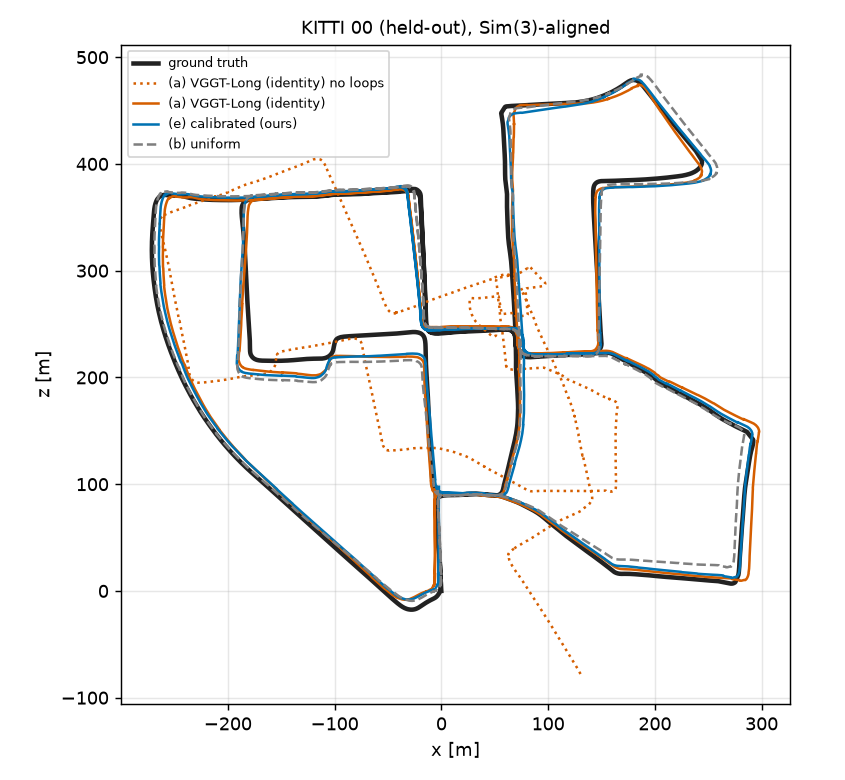
\includegraphics[width=\textwidth]{trajectory_00.png}\end{subfigure}
\begin{subfigure}{0.49\textwidth}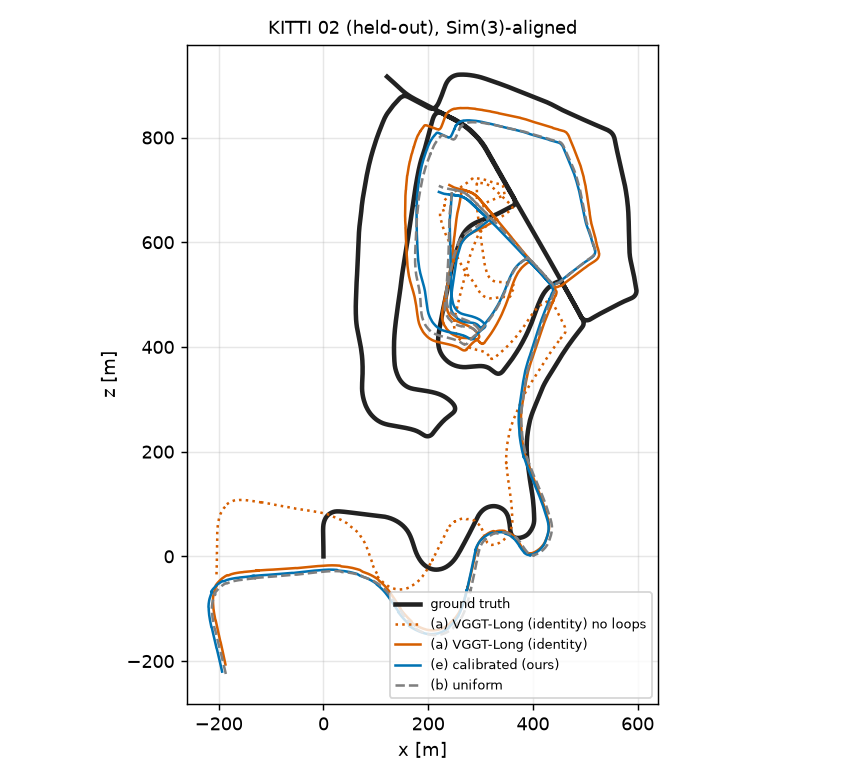
\includegraphics[width=\textwidth]{trajectory_02.png}\end{subfigure}
\caption{Held-out trajectories (top view, m). On 00 loops pull the drifting chain (dotted) onto the ground truth. On 02 all
loops join the start of the drive to its end, so the long middle section keeps its drift.}
\label{fig:traj}
\end{figure}

\begin{figure}[H]
\centering
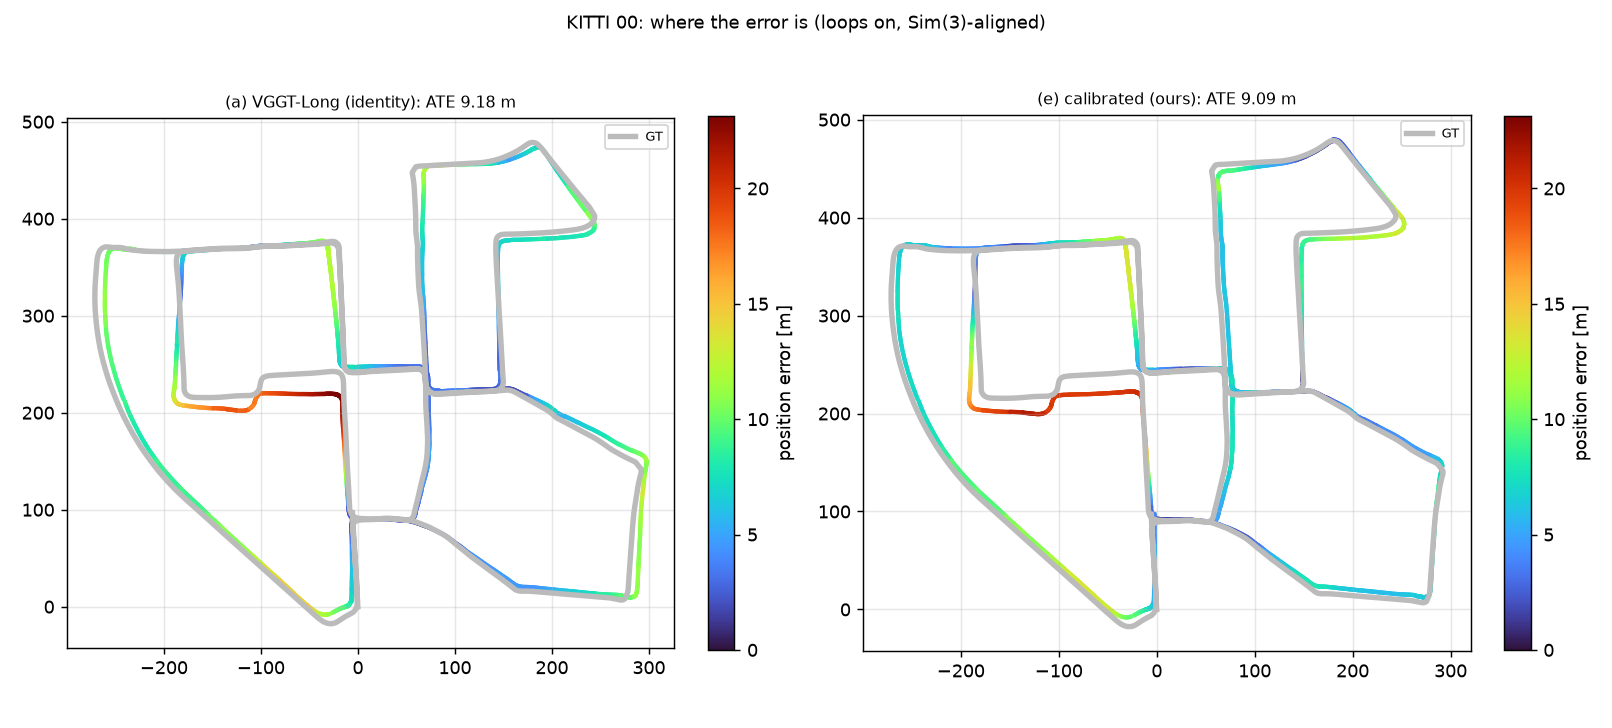
\includegraphics[width=0.85\textwidth]{trajectory_error_00.png}
\caption{KITTI 00, position error along the path with VGGT-Long's weights (left) and ours (right). The largest error (about
20\,m) is on a detour that no loop closes; our weights lower the error on most other parts.}
\label{fig:trajerr}
\end{figure}

\begin{figure}[H]
\centering
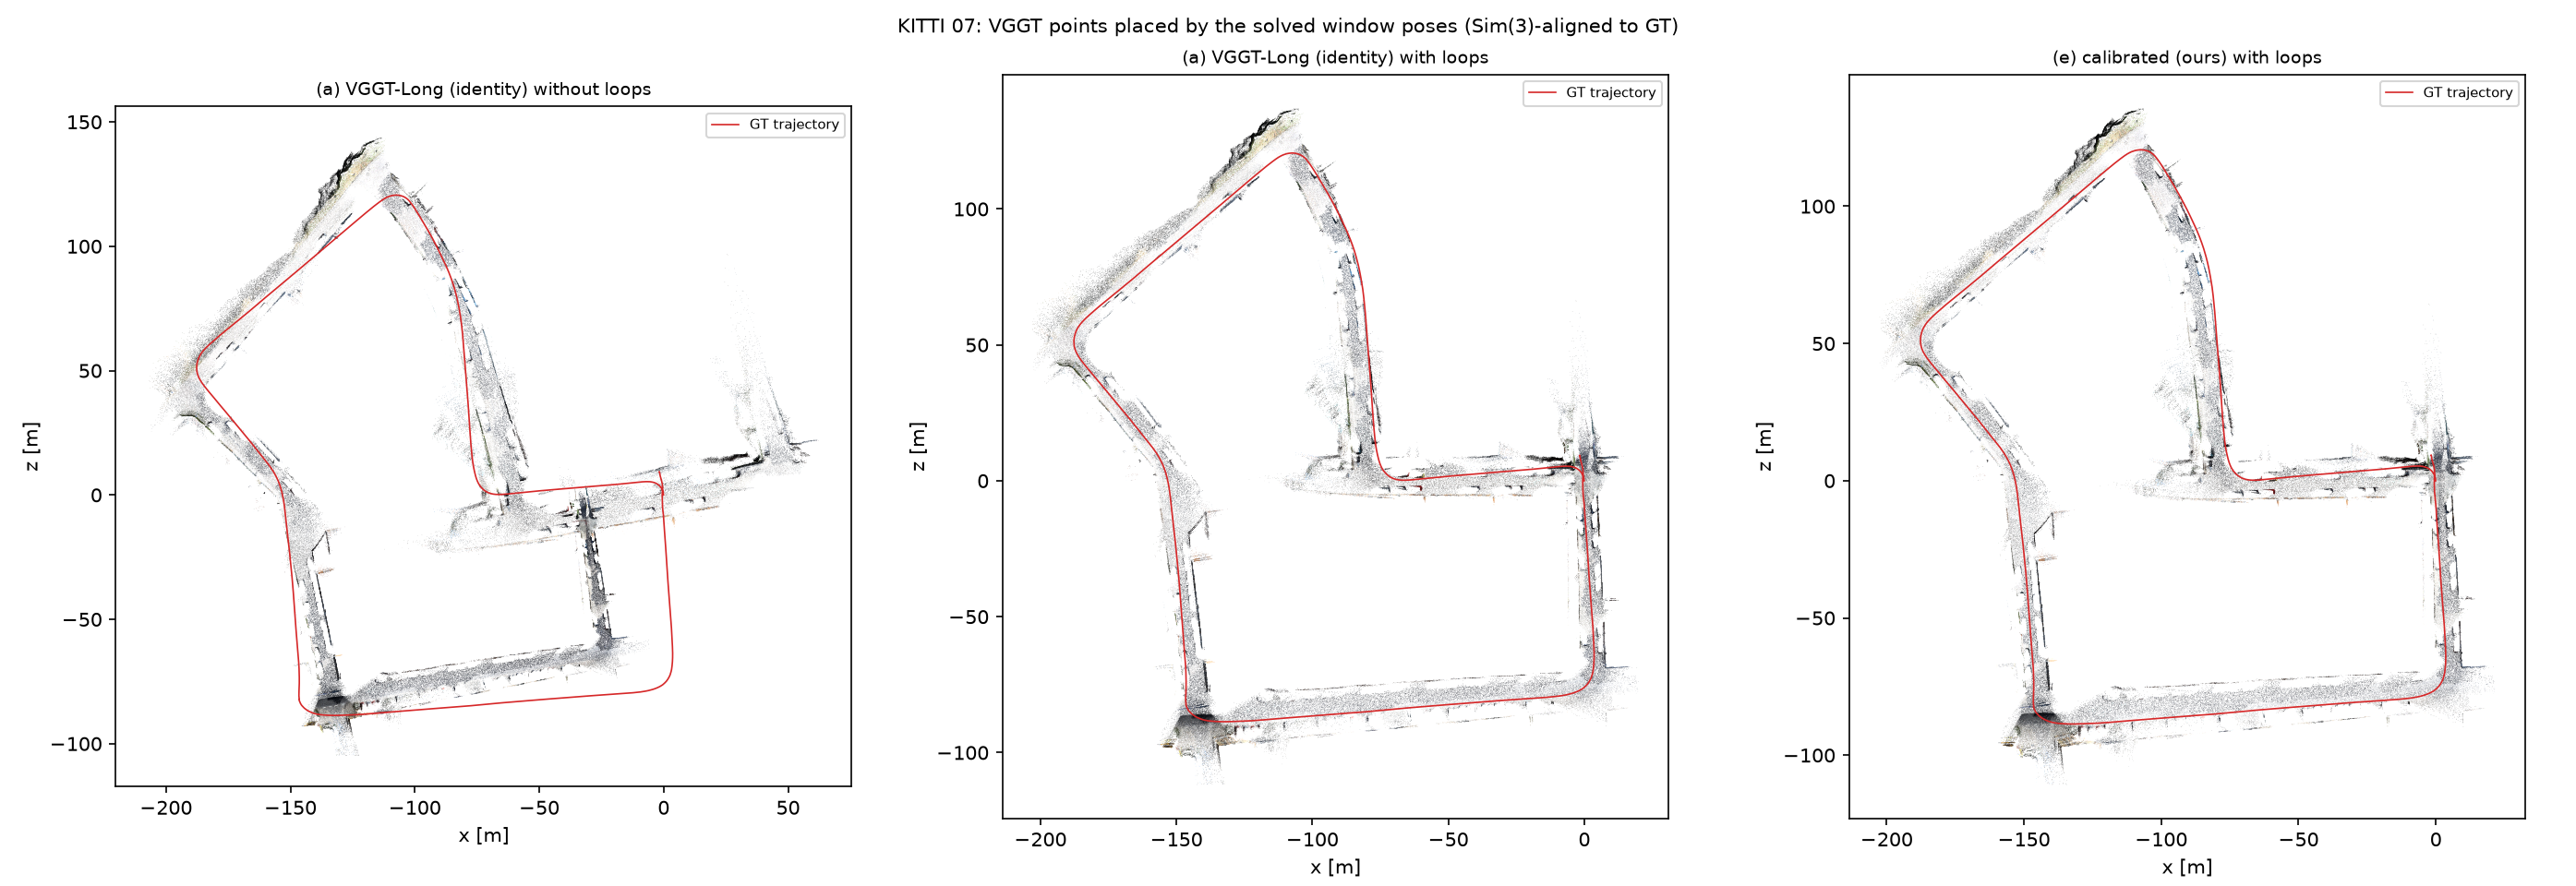
\includegraphics[width=\textwidth]{pointcloud_07.png}
\caption{KITTI 07, VGGT's points placed by the solved window poses (top view; true path in red). Without loops the map does
not close; with loops (VGGT-Long's weights, middle, and ours, right) it does.}
\label{fig:pc}
\end{figure}

\subsection{Summary of findings}
\begin{itemize}
  \item VGGT-Long is reproduced: the original code matches the paper, and our version matches the original code.
  \item Pixel confidence is a reliable ranking of depth error and becomes a good error estimate after calibration.
  \item Averaging confidence over a seam keeps information about rotation but loses most of it about translation.
  \item KITTI's ground truth is inconsistent in height (up to 4\,m) at the revisits of 02 and, less so, 00, which we
        confirmed with LiDAR. Loop errors measured against it on those sequences are therefore mostly ground-truth error.
  \item At the trajectory level, calibrated weights so far give small gains on some sequences (05, 00, against the fair
        control) and losses on others (07, 02); window size and loop closures matter more than edge weights.
\end{itemize}

\section{Plans for further improvements and development}

\begin{itemize}
  \item \textbf{False-loop stress test:} add 1 to 16 wrong loops between distant windows and compare how the weighting
        schemes and robust kernels survive.
  \item \textbf{More data and baselines:} Waymo Open Dataset and TUM RGB-D sequences; ORB-SLAM3 (monocular) as a classical
        reference; a memory and speed comparison; MASt3R-SLAM if time allows.
  \item \textbf{Bonus:} streaming models (CUT3R, StreamVGGT) and VGGT-$\Omega$ in the same pipeline.
\end{itemize}

\begin{thebibliography}{9}
\bibitem{vggt} J.~Wang, M.~Chen, N.~Karaev, A.~Vedaldi, C.~Rupprecht, and D.~Novotny, ``VGGT: Visual geometry grounded
transformer,'' in \emph{Proc. CVPR}, 2025.
\bibitem{vggtlong} K.~Deng, Z.~Ti, J.~Xu, J.~Yang, and J.~Xie, ``VGGT-Long: Chunk it, loop it, align it: Pushing VGGT's
limits on kilometer-scale long RGB sequences,'' \emph{arXiv:2507.16443}, 2025.
\bibitem{dengaudit} N.~N.~Deng, Q.~Cheng, N.~Zeller, and D.~Cremers, ``A calibration audit of confidence in feed-forward
3D reconstruction models,'' arXiv:2608.29705v3, 2026.
\bibitem{kitti} A.~Geiger, P.~Lenz, and R.~Urtasun, ``Are we ready for autonomous driving? The KITTI vision benchmark
suite,'' in \emph{Proc. CVPR}, 2012.
\bibitem{dcs} P.~Agarwal, G.~D.~Tipaldi, L.~Spinello, C.~Stachniss, and W.~Burgard, ``Robust map optimization using
dynamic covariance scaling,'' in \emph{Proc. ICRA}, 2013.
\bibitem{umeyama} S.~Umeyama, ``Least-squares estimation of transformation parameters between two point patterns,''
\emph{IEEE TPAMI}, 13(4):376--380, 1991.
\bibitem{evo} M.~Grupp, ``evo: Python package for the evaluation of odometry and SLAM,''
\url{https://github.com/MichaelGrupp/evo}, 2017.
\end{thebibliography}

\end{document}
